%%%%%%%%%%%%%%%%%%%%%%%%%%%%%%%%%%%%%%%%%%%%%%%%%%%%%%%%
%                IAML 2020 Assignment 2                %
%                                                      %
%                                                      %
% Authors: Hiroshi Shimodaira and JinHong Lu           %
% Based on: Assignment 1 by Oisin Mac Aodha, and       %
%          Octave Mariotti                             %
% Using template from: Michael P. J. Camilleri and     %
% Traiko Dinev.                                        %
%                                                      %
% Based on the Cleese Assignment Template for Students %
% from http://www.LaTeXTemplates.com.                  %
%                                                      %
% Original Author: Vel (vel@LaTeXTemplates.com)        %
%                                                      %
% License:                                             %
% CC BY-NC-SA 3.0                                      %
% (http://creativecommons.org/licenses/by-nc-sa/3.0/)  %
%                                                      %
%%%%%%%%%%%%%%%%%%%%%%%%%%%%%%%%%%%%%%%%%%%%%%%%%%%%%%%%

%--------------------------------------------------------
%   IMPORTANT: Do not touch anything in this part
\documentclass[12pt]{article}
\input{style.tex}



% Options for Formatting Output

\global\setbool{clearon}{true} %
\global\setbool{authoron}{true} %
\ifbool{authoron}{\rhead{\small{\assignmentAuthorName}}\cfoot{\small{\assignmentAuthorName}}}{\rhead{}}



\newcommand{\assignmentQuestionName}{Question}
\newcommand{\assignmentTitle}{Assignment\ \#2}

\newcommand{\assignmentClass}{IAML -- INFR10069 (LEVEL 10)}

\newcommand{\assignmentWarning}{NO LATE SUBMISSIONS} % 
\newcommand{\assignmentDueDate}{Monday,\ November\ 23,\ 2020 @ 16:00}
%--------------------------------------------------------



%%%%%%%%%%%%%%%%%%%%%%%%%%%%%%%%%%%%%%%%%%%%%%%%%%%%%%%
%
% NOTE: YOU NEED TO ENTER YOUR STUDENT ID BELOW.
%
%%%%%%%%%%%%%%%%%%%%%%%%%%%%%%%%%%%%%%%%%%%%%%%%%%%%%%%% 
% --------------------------------------------------------
% IMPORTANT: Specify your Student ID below. You will need to uncomment the line, else compilation will fail. Make sure to specify your student ID correctly, otherwise we may not be able to identify your work and you will be marked as missing.
\newcommand{\assignmentAuthorName}{s1720422}
%--------------------------------------------------------



\begin{document}


%%%%%%%%%%%%%%%%%%%%%%%%%%%%%%%%%%%%%%%%%%%%%%%%%%%%%%%%%%%%%%%%%%%%%%%%%%%%%%
%============================================================================%
%%%%%%%%%%%%%%%%%%%%%%%%%%%%%%%%%%%%%%%%%%%%%%%%%%%%%%%%%%%%%%%%%%%%%%%%%%%%%%
\clearpage
%
% Question 1
%

\begin{question}{(30 total points) Image data analysis with PCA}

  
  \questiontext{In this question we employ PCA to analyse image data}
  

  
  \medskip

   %==============================
   % Q1.1
  \begin{subquestion}{(3 points)
      Once you have applied the normalisation from Step 1 to Step 4 above,
      report the values of the first 4 elements for the first training
      sample in \texttt{Xtrn\_nm},
      i.e. \texttt{Xtrn\_nm[0,:]} and the last training sample,
      i.e. \texttt{Xtrn\_nm[-1,:]}.
    } \label{Q1.1}
    

      \begin{answerbox}{10em}
         For the first and last training samples, the values of the first 4 elements are the exact same and as follows:\newline
         Element 1: $-3.137\times10^{-6}$\newline
         Element 2: $-2.268\times10^{-6}$\newline
         Element 3: $-1.180\times10^{-6}$\newline
         Element 4: $-4.071\times10^{-6}$\newline
      \end{answerbox}
  


   \end{subquestion}
   %
   % ==============================
   % 
   % Q1.2
   \begin{subquestion}{(4 points)
      Using {\tt Xtrn} and Euclidean distance
      measure, for each class,
      find the two closest samples and two furthest
      samples of that class to the mean vector of the class.
    }  \label{Q1.2}




  \begin{answerbox}{52em}
    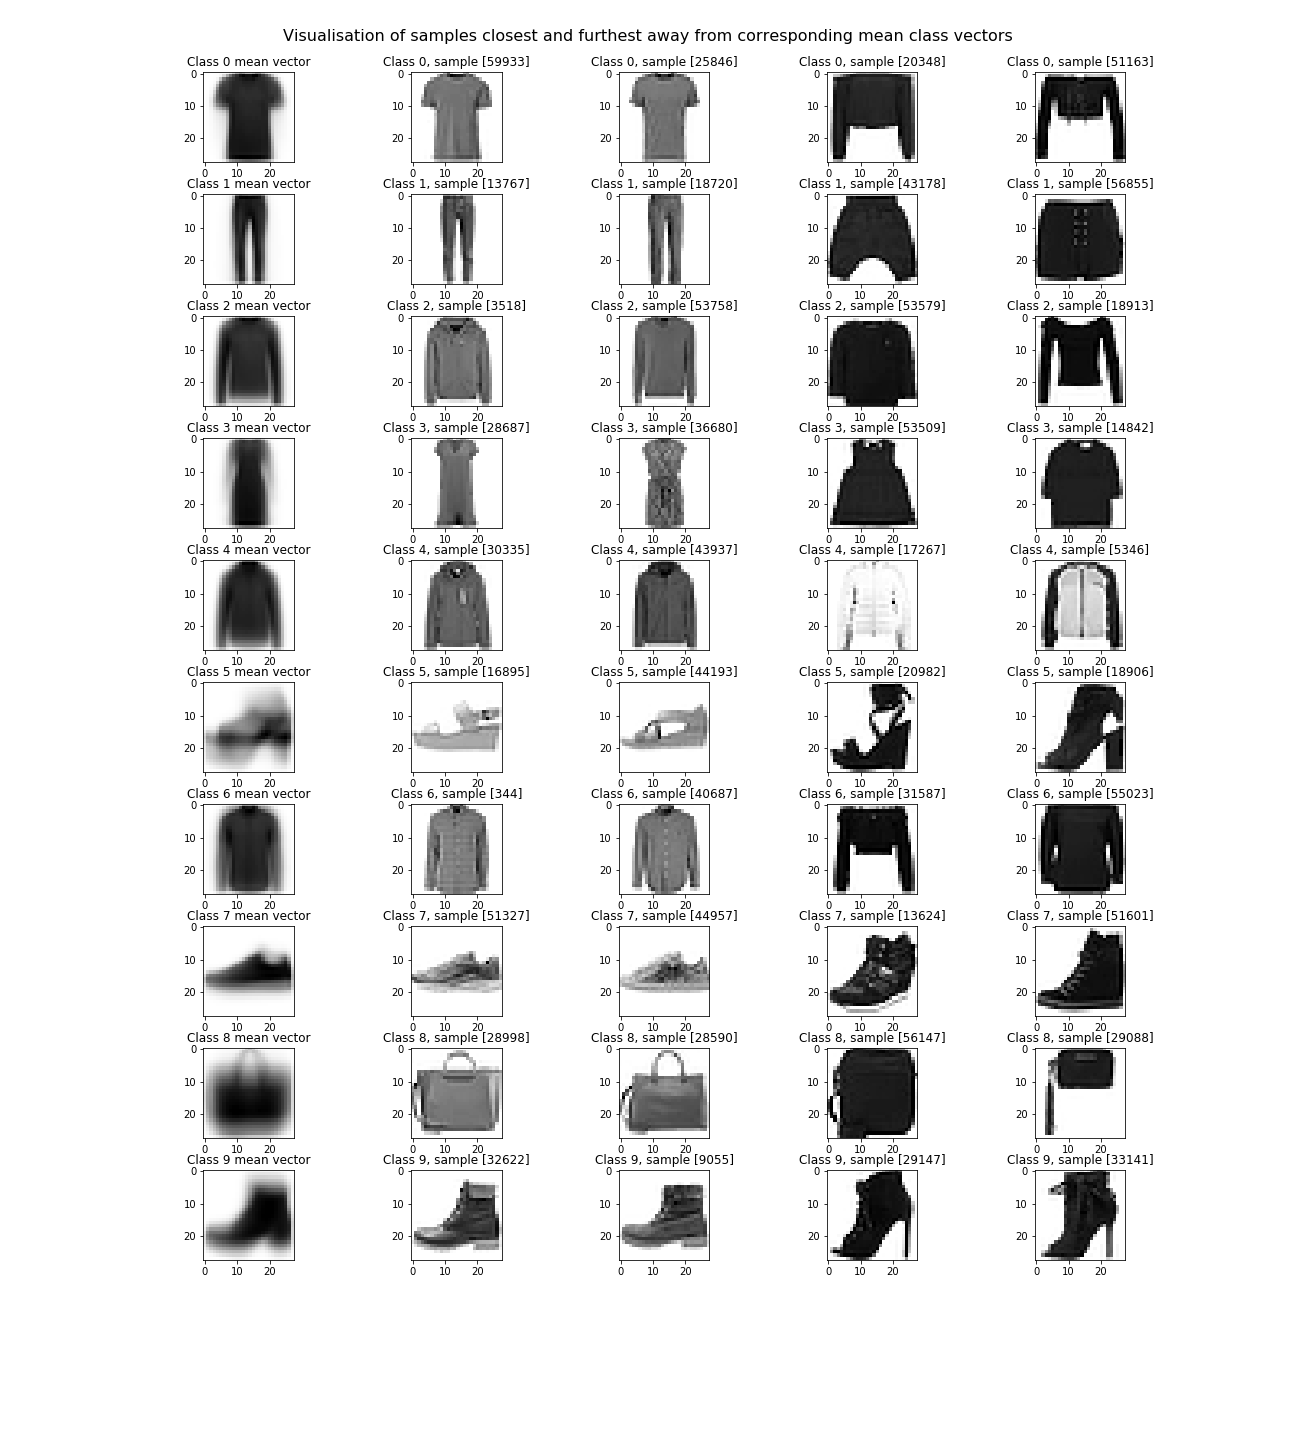
\includegraphics[width = 1.0\textwidth]{q1_2.png}
    By visualising the data, we can see that the samples with a smaller Euclidean Distance away from the mean vector tend to resemble the class of the mean vector a lot more than samples which are further away from the mean vector. One prime example being in class 1. The actual class is for trousers, however the samples furthest away from the mean vector resemble shorts.
  \end{answerbox}



   \end{subquestion}

   % 
   % Q1.3
   \begin{subquestion}{(3 points)
       Apply Principal Component Analysis (PCA) to the data of {\tt
         Xtrn\_nm} using
       \href{https://scikit-learn.org/0.19/modules/generated/sklearn.decomposition.PCA.html}{sklearn.decomposition.PCA},
       and report the variances of projected data for the first five principal
       components in a table. 
       Note that you should use {\tt Xtrn\_nm} instead of {\tt Xtrn}.
           } \label{Q1.pca.variance}



    \begin{answerbox}{15em}
    \begin{center}
    \caption{Variance of first 5 principal components}\newline
    \begin{tabular}{c|c|c|c|c}
    \hline
    Component 1 & Component 2 & Component 3 & Component 4 & Component 5 \\ \hline
    19.81 & 12.11 & 4.106 & 3.382 & 2.625 \\
    \hline
    \end{tabular}
    \end{center}
      
    \end{answerbox}
    


   \end{subquestion}

   %==============================
   % Q1.4
   \begin{subquestion}{(3 points)
       Plot a graph of the cumulative explained variance ratio as a
       function of the number of principal components, $K$, where $1
       \le K \le 784$.
       Discuss the result briefly.
     } \label{Q1.plot.pca.variance}
   

      \begin{answerbox}{30em}
        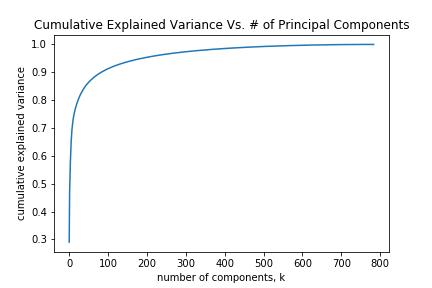
\includegraphics[width = 1.0\textwidth]{q1_4.png}
        It can be seen that as the number of components being used is increased up until k = 150, the amount of variance accounted for within the data rapidly increases.Beyond that point, the total variance doesn't increase much as k is increased.
    
      \end{answerbox}
  


   \end{subquestion}

   %==============================
   % Q1.5
   \begin{subquestion}{(4 points)
      Display the images of the first 10 principal components in
      a 2-by-5 grid, putting the image of 1st principal component on
      the top left corner, followed by the one of 2nd component to the right.
      Discuss your findings briefly.
     } \label{Q1.disp.pca}
   

      \begin{answerbox}{35em}
         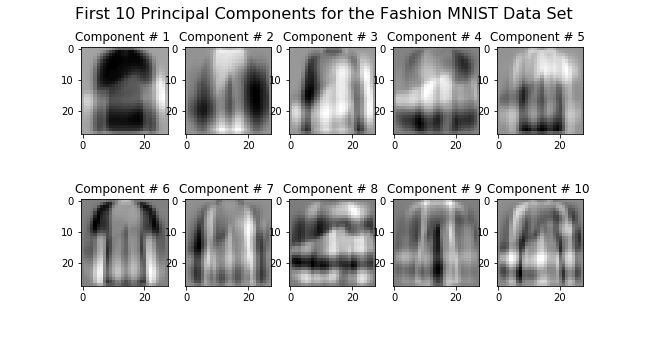
\includegraphics[width = 1.0\textwidth]{q1_5.png}
         From the above results it can be deduced that PCA has managed to capture the representation of most classes fairly well. For example, class 0 is meant to be a top which has its outline captured in black by the first component. Similarly, component 2 captures the trouser class (1) fairly well as indicated by the white outline of the component image. However the representation of classes become diluted for components which represent a lower variance. This can be seen with component 6 which should represent a sandal but shows no pattern corresponding to that item.
         
      \end{answerbox}
  


   \end{subquestion}

   %==============================
   % Q1.6
   \begin{subquestion}{(5 points)
       Using \texttt{Xtrn\_nm}, 
       for each class and for each number of principal components $K =
       5, 20, 50, 200$, apply dimensionality reduction with PCA to the
       first sample in the class, reconstruct the sample from the
       dimensionality-reduced sample, and 
       report the Root Mean Square Error (RMSE) between the
       original sample in {\tt Xtrn\_nm} and reconstructed one.
     } \label{Q1.6}

     

      \begin{answerbox}{25em}
         \begin{center}
        \caption{RMSE values for table of Class$\times$\# of components(k)}\newline
        \begin{tabular}{c|c|c|c|c}
        \hline
        Class & k = 5 & k = 20 & k = 50 & k = 200 \\ \hline
        0 & 0.2561 & 0.1502 & 0.1275 & 0.0613 \\
        1 & 0.1980 & 0.1404 & 0.0955 & 0.0347 \\
        2 & 0.1987 & 0.1454 & 0.1237 & 0.0821 \\
        3 & 0.1457 & 0.1073 & 0.0831 & 0.0567 \\
        4 & 0.1182 & 0.1027 & 0.0878 & 0.0468 \\
        5 & 0.1811 & 0.1590 & 0.1423 & 0.0899 \\
        6 & 0.1295 & 0.0957 & 0.0722 & 0.0459 \\
        7 & 0.1656 & 0.1280 & 0.1069 & 0.0637 \\
        8 & 0.2234 & 0.1451 & 0.1235 & 0.0923 \\
        9 & 0.1835 & 0.1518 & 0.1221 & 0.0711 \\
        \hline
        \end{tabular}
        \end{center}
      \end{answerbox}
  


   \end{subquestion}
   
   %==============================
   % Q1.7
   \begin{subquestion}{(4 points)
       Display the image for each of the reconstructed samples in
       a 10-by-4 grid, where each row corresponds to a class and
       each row column corresponds to a value of $K=5, \; 20, \; 50, \; 200$.
     } \label{Q1.7}


   

      \begin{answerbox}{52em}
         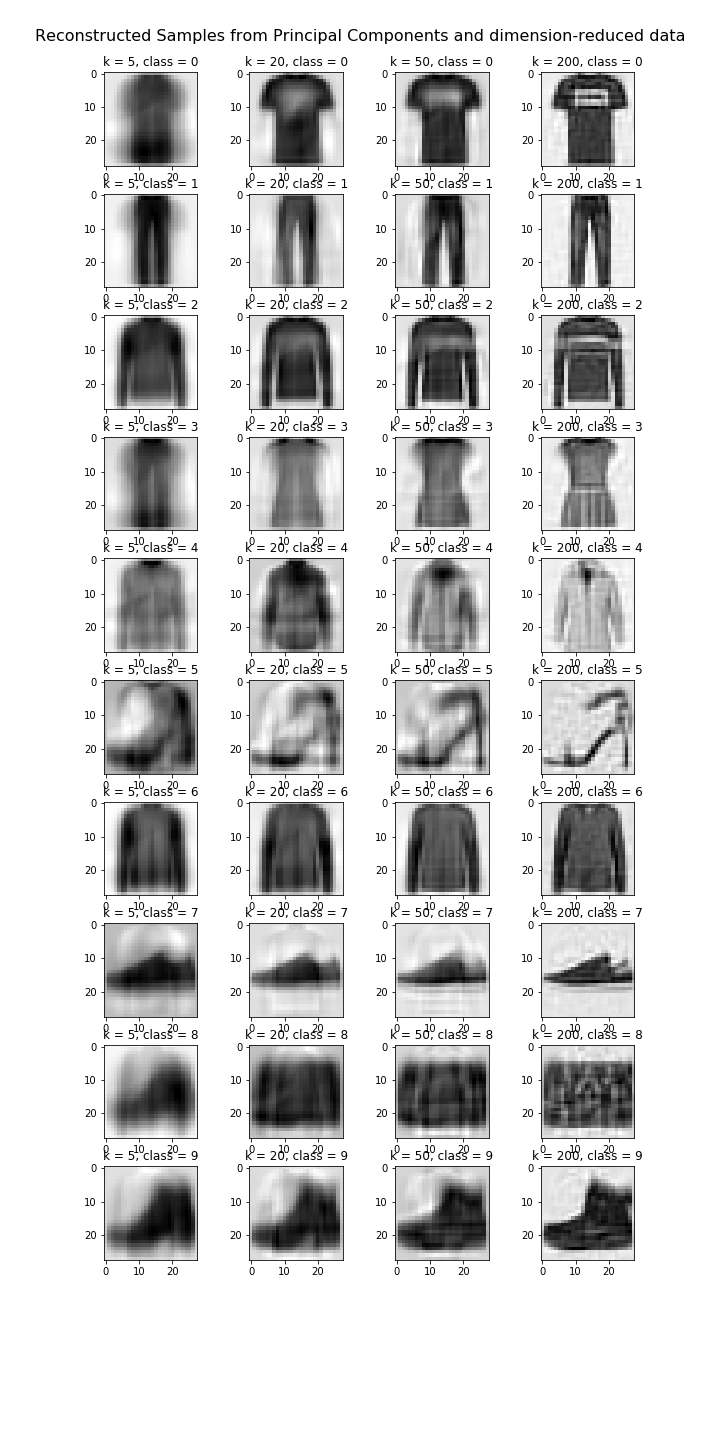
\includegraphics[width = 0.63\textwidth]{q1_7.png}
         From the plot above, it can be seen that as the number of principal components increase, the clarity of the reconstructed sample improves and looks more like a specific piece of clothing. The reason for this is due to a larger variance of the complete data being accounted for when higher values of k are used.
      \end{answerbox}
  


   \end{subquestion}
   %==============================
   %
   %==============================
   % Q1.8
   \begin{subquestion}{(4 points)
       Plot all the training samples (\texttt{Xtrn\_nm}) on the
       two-dimensional PCA plane you obtained in \refQ{Q1.pca.variance}, where each sample is
       represented as a small point with a colour specific to the class of
       the sample.  Use the 'coolwarm' colormap for plotting.
     } \label{Q1.8}


   

      \begin{answerbox}{40em}
         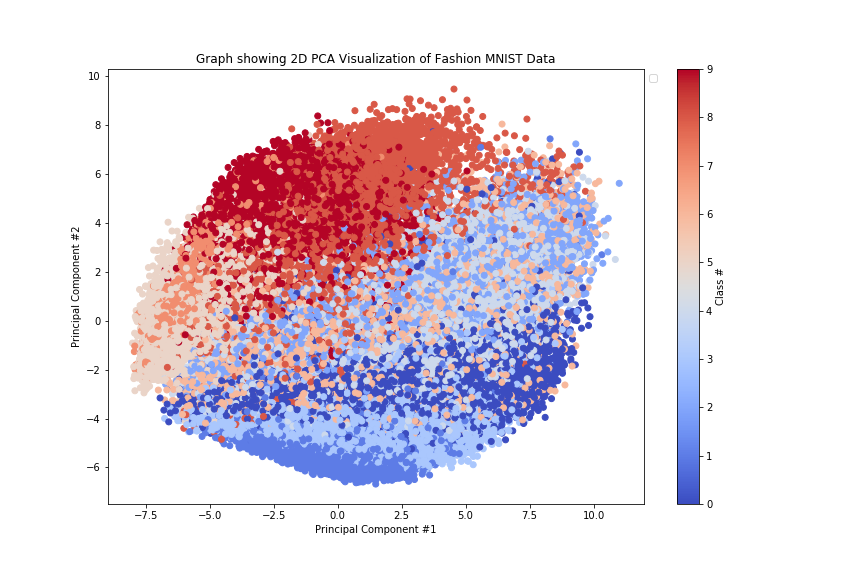
\includegraphics[width = 1.0\textwidth]{q1_8.png}
         From the plot above we can deduce that class 9 an class 6 are well defined by their own clusters, densely distributed and are mostly separable. Whereas points belonging to class 4,2 and 8 tend to be very spread out and hard to separate from other classes. The remaining classes tend to be mostly separable on the outer edges of the overall cluster.
      \end{answerbox}
  


   \end{subquestion}
   %
   %==============================
   

\end{question}
%%%%%%%%%%%%%%%%%%%%%%%%%%%%%%%%%%%%%%%%%%%%%%%%%%%%%%%%%%%%%%%%%%%%%%%%%%%%%%
%============================================================================%
%%%%%%%%%%%%%%%%%%%%%%%%%%%%%%%%%%%%%%%%%%%%%%%%%%%%%%%%%%%%%%%%%%%%%%%%%%%%%%
\clearpage
%
% Question 2
%
\begin{question}{(25 total points) Logistic regression and SVM}

  \questiontext{In this question we will explore 
    classification of image data with logistic regression and support
    vector machines (SVM) and visualisation 
    of decision regions.
  }
  


  \medskip
   %==============================
   % Q2.1
   \begin{subquestion}{(3 points)
       Carry out a classification experiment with
       \href{https://scikit-learn.org/0.19/modules/generated/sklearn.linear\_model.LogisticRegression.html}{multinomial logistic regression},
       and report the classification accuracy and confusion matrix (in
       numbers rather than in graphical representation such as heatmap)
       for the test set.
     } \label{Q2.1}


   

    \begin{answerbox}{30em}
    Testing Accuracy: 84.01\%\newline
    \centreline{Table showing confusion matrix for Actual Classes Vs. Predicted Classes.}\newline
    \centerline{Predicted Classes}
    \begin{center}
    \begin{tabular}{c|c|c|c|c|c|c|c|c|c}
    \hline
    \multicolumn{1}{c}{\bfseries 0} & \multicolumn{1}{c}{\bfseries 1} & \multicolumn{1}{c}{\bfseries 2} & \multicolumn{1}{c}{\bfseries 3} &
    \multicolumn{1}{c}{\bfseries 4} & \multicolumn{1}{c}{\bfseries 5} &
    \multicolumn{1}{c}{\bfseries 6} & \multicolumn{1}{c}{\bfseries 7} &
    \multicolumn{1}{c}{\bfseries 8} & \multicolumn{1}{c}{\bfseries 9} \\ \hline
    819 & 3   & 15  & 50  & 7   & 4   & 90  & 1   & 11  & 0   \\ 
    5      & 953 & 4   & 27  & 5   & 0   & 3   & 1   & 2   & 0   \\ 
    27     & 4   & 731 & 11  & 133 & 0   & 82  & 2   & 9   & 11  \\ 
    31     & 15  & 14  & 866 & 33  & 0   & 37  & 0   & 4   & 0   \\ 
    0      & 3   & 115 & 38  & 760 & 2   & 72  & 0   & 10  & 0   \\ 
    2      & 0   & 0   & 1   & 0   & 911 & 0   & 56  & 10  & 20  \\ 
    147    & 3   & 128 & 46  & 108 & 0   & 539 & 0   & 28  & 1   \\ 
    0      & 0   & 0   & 0   & 0   & 32  & 0   & 936 & 1   & 31  \\ 
    7      & 1   & 6   & 11  & 3   & 7   & 15  & 5   & 945 & 0   \\ 
    0      & 0   & 0   & 1   & 0   & 15  & 1   & 42  & 0   & 941 \\ 
    \hline
    \end{tabular}
    \end{center}          
    
    \end{answerbox}
  


   \end{subquestion}
   %
   % ==============================
   %
   %==============================
   % Q2.2
   \begin{subquestion}{(3 points)
       Carry out a classification experiment with
       \href{https://scikit-learn.org/0.19/modules/generated/sklearn.svm.SVC.html}{SVM classifiers}, and report the
       mean accuracy and confusion matrix (in numbers) for the test
       set.
     } \label{Q2.2}


   

      \begin{answerbox}{30em}
         Testing Accuracy: 84.61\%\newline
             \centreline{Table showing confusion matrix for Actual Classes Vs. Predicted Classes.}\newline
        \centerline{Predicted Classes}
        \begin{center}
        \begin{tabular}{c|c|c|c|c|c|c|c|c|c}
        \hline
        \multicolumn{1}{c}{\bfseries 0} & \multicolumn{1}{c}{\bfseries 1} & \multicolumn{1}{c}{\bfseries 2} & \multicolumn{1}{c}{\bfseries 3} &
        \multicolumn{1}{c}{\bfseries 4} & \multicolumn{1}{c}{\bfseries 5} &
        \multicolumn{1}{c}{\bfseries 6} & \multicolumn{1}{c}{\bfseries 7} &
        \multicolumn{1}{c}{\bfseries 8} & \multicolumn{1}{c}{\bfseries 9} \\ \hline
        845    & 2   & 8  & 51  & 4   & 4   & 72  & 0   & 14  & 0   \\ 
        4      & 951 & 7   & 31  & 5   & 0   & 1   & 0   & 1   & 0   \\ 
        15     & 2   & 748 & 11  & 137 & 0   & 79  & 0   & 8   & 0  \\ 
        32     & 6  & 12  & 881 & 26  & 0   & 40  & 0   & 3   & 0   \\ 
        1      & 0   & 98 & 36  & 775 & 0   & 86  & 0   & 4  & 0   \\ 
        0      & 0   & 0   & 1   & 0   & 914 & 0   & 57  & 2  & 26  \\ 
        185    & 1   & 122 & 39  & 95 & 0   & 533 & 0   & 25  & 0   \\ 
        0      & 0   & 0   & 0   & 0   & 34  & 0   & 925 & 0   & 41  \\ 
        3      & 1   & 8   & 5  & 2   & 4   & 13  & 4   & 959 & 1   \\ 
        0      & 0   & 0   & 0   & 0   & 22  & 0   & 47  & 1   & 930 \\ 
        \hline
        \end{tabular}
        \end{center}      
         
      \end{answerbox}
  


   \end{subquestion}
   %
   % ==============================
   %
   %==============================
   % Q2.3
   \begin{subquestion}{(6 points)
       We now want to visualise the decision regions for the logistic
       regression classifier we trained in \refQ{Q2.1}.
     } \label{Q2.3}


   

      \begin{answerbox}{35em}
         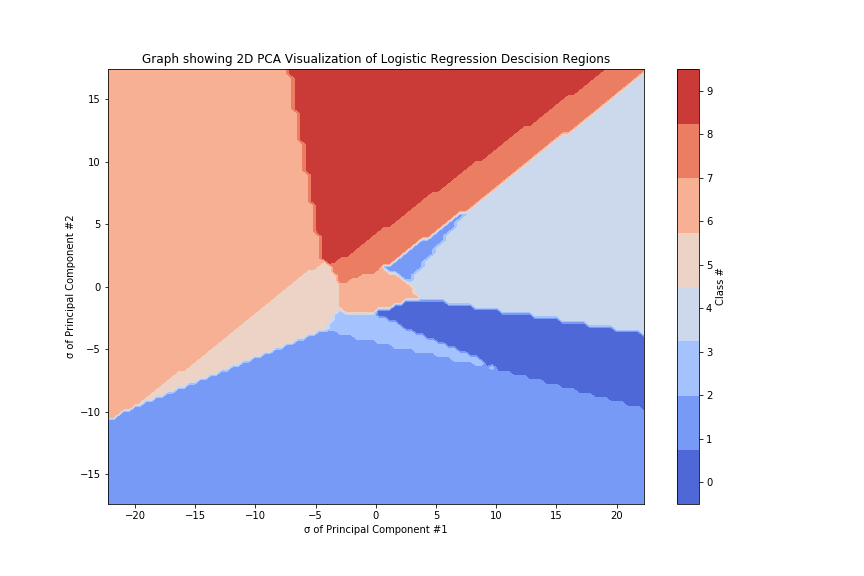
\includegraphics[width = 1.0\textwidth]{q2_3.png}
         From the plot above we can see that there are 10 distinct regions for each class which are all separated by a linear boundary.
      \end{answerbox}
  


   \end{subquestion}
   %
   % ==============================
   %
   %==============================
   % Q2.4
   \begin{subquestion}{(4 points)
       Using the same method as the one above, plot the decision regions for
       the SVM classifier you trained in \refQ{Q2.2}.
       Comparing the result with that you obtained in \refQ{Q2.3}, discuss your
       findings briefly.
     } \label{Q2.4}
   

      \begin{answerbox}{35em}
         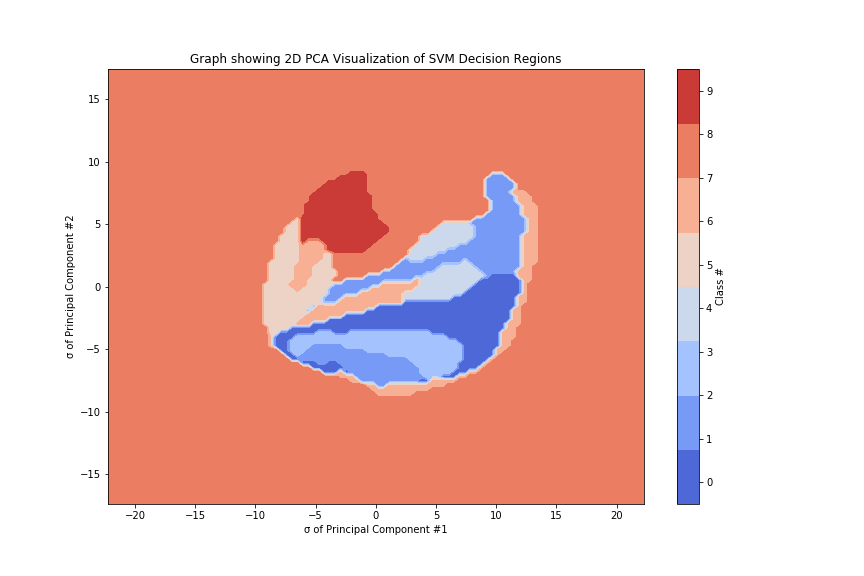
\includegraphics[width = 1.0\textwidth]{q2_4.png}
         From the plot above we can see that the decision regions for the SVM classifier are non-linear. This is due to the RBF kernel being employed which maps points to areas based on how far they are from the centre of the radial basis function. Hence this results in non-linear decision boundaries. Furthermore, nearly all of the decision regions are centrally located and confined within a smaller space compared to the Logistic regression classifier which has it's decision boundaries distributed across the entire plot.
      \end{answerbox}
  


   \end{subquestion}
   %
   % ==============================
   %

   %==============================
   % Q2.5
   \begin{subquestion}{(6 points)
       We used default parameters for the SVM in \refQ{Q2.2}.
       We now want to tune the parameters by using cross-validation.
       To reduce the time for experiments, you pick up the first 1000
       training samples from each class to create \texttt{Xsmall}, so that \texttt{Xsmall}
       contains 10,000 samples in total. Accordingly, you create
       labels, \texttt{Ysmall}.
     } \label{Q2.5}


   

      \begin{answerbox}{30em}
         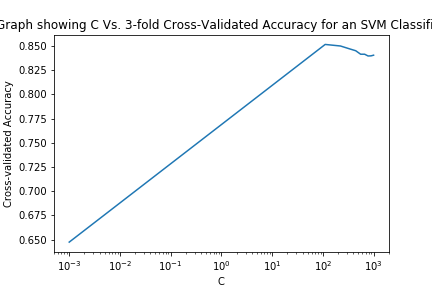
\includegraphics[width = 1.0\textwidth]{q2_5.png}
         From the graph above we can see that when c = 100, we obtain the highest mean accuracy score of approximately 84.0\%. 
         
      \end{answerbox}
  


   \end{subquestion}
   %
   % ==============================
   %
   %==============================
   % Q2.6
   \begin{subquestion}{(3 points)
       Train the SVM classifier on the whole training set by using the
       optimal value of $C$ you found in \refQ{Q2.5}. 
     } \label{Q2.6}


       

      \begin{answerbox}{10em}
         Given C = 100,\newline
         Training set accuracy: 93.82\%\newline
         Testing set accuracy: 88.04\%
      \end{answerbox}
  


   \end{subquestion}
   %
   % ==============================
   %
%
%

\end{question}
%%%%%%%%%%%%%%%%%%%%%%%%%%%%%%%%%%%%%%%%%%%%%%%%%%%%%%%%%%%%%%%%%%%%%%%%%%%%%%
%============================================================================%
%%%%%%%%%%%%%%%%%%%%%%%%%%%%%%%%%%%%%%%%%%%%%%%%%%%%%%%%%%%%%%%%%%%%%%%%%%%%%%
\clearpage
%
% Question 3
%

\begin{question}{(20 total points) Clustering and Gaussian Mixture Models}  


  \questiontext{In this question we will explore K-means clustering,
    hierarchical clustering, and GMMs.
  }
  


  \medskip
   %==============================
   % Q3.1
   \begin{subquestion}{(3 points)
       Apply k-means clustering on {\tt Xtrn} for $k = 22$, where we use
       \href{https://scikit-learn.org/0.19/modules/generated/sklearn.cluster.KMeans.html}{sklearn.cluster.KMeans}
       with the parameters {\tt n\_clusters=22} and {\tt random\_state=1}.
       Report the sum of squared distances of samples to their closest
       cluster centre, and the number of samples for each cluster.
     } \label{Q3.1}
   

      \begin{answerbox}{35em}
         Inertia = 38185.82
            \begin{center}
    \caption{   Table showing amount of samples assigned to each cluster}\newline
    \begin{tabular}{c|c}
    \hline
    Cluster \# & \# of Samples \\ \hline
    0 & 1018 \\
    1 & 1125  \\
    2 & 1191 \\
    3 & 890 \\
    4 & 1162 \\
    5 & 1332 \\
    6 & 839  \\
    7 & 623 \\
    8 & 1400 \\
    9 & 838 \\
    10 & 659 \\
    11 & 1276 \\
    12 & 121 \\
    13 & 152 \\
    14 & 950 \\
    15 & 1971 \\
    16 & 1251 \\
    17 & 845 \\
    18 & 896 \\
    19 & 930 \\
    20 & 1065 \\
    21 & 1466 \\
    
    \hline
    \end{tabular}
    \end{center}
      \end{answerbox}
  


   \end{subquestion}
   %
   % ==============================
   %
   %==============================
   % Q3.2
   \begin{subquestion}{(3 points)
       Using the training set only,
       calculate the mean vector for each language, and plot the mean
       vectors of all the 22 languages on a 2D-PCA plane, where you
       apply PCA on the set of 22 mean vectors without applying
       standardisation.  
       On the same figure, plot the cluster centres obtained in \refQ{Q3.1}.
     } \label{Q3.2}

   

      \begin{answerbox}{35em}
         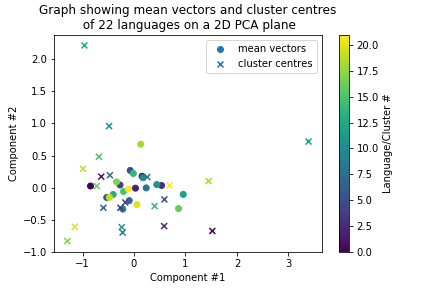
\includegraphics[width = 1.0\textwidth]{q3_2.png}
         From the plot above it can be seen that the mean vectors for languages tend to be grouped closer together, whereas the cluster centres for each language tend to be more spread out. Generally, the mean vectors and cluster centres are distributed in similar areas apart from a few outliers located at the top left and far right of the plot.
      \end{answerbox}
  


   \end{subquestion}
   %
   % ==============================
   %
   %==============================
   % Q3.3
   \begin{subquestion}{(3 points)
       We now apply hierarchical clustering on the training data set
       to see if there are any structures in the spoken languages.
     } \label{Q3.3}


     

      \begin{answerbox}{35em}
         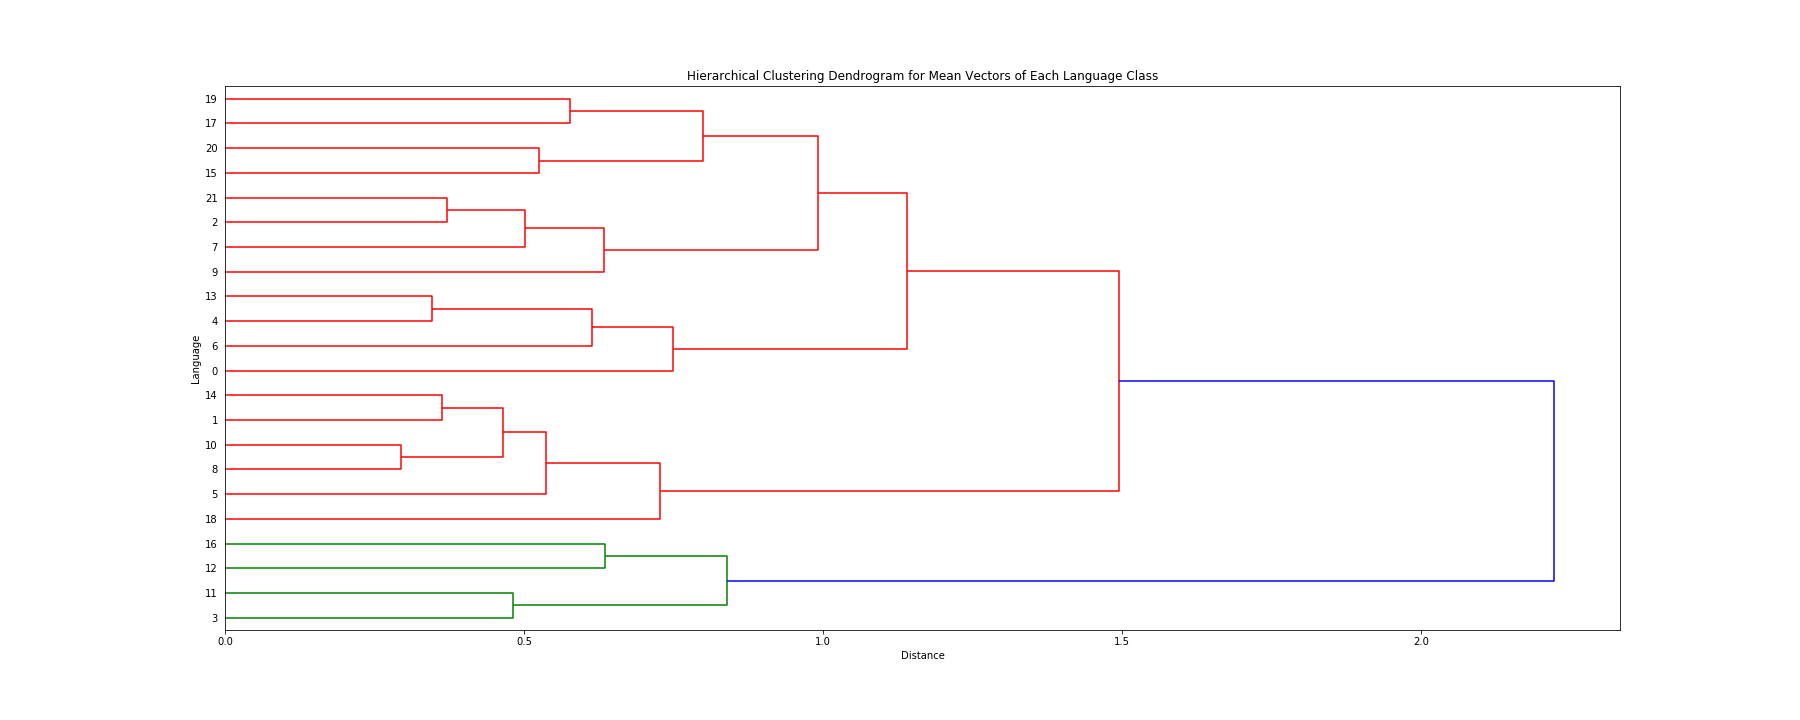
\includegraphics[width=15cm, height=11cm]{q3_3.png}
         From the dendrogram above it can be seen that languages 16, 12, 11 and 3 are very distinct compared to the rest of the languages. This is because the distance required to merge them with the red cluster is very large.An appropriate cut-off distance would be at around d = 0.85 where we would have 5 clusters. Beyond that, a large distance is needed for the next merge to occur.
         
      \end{answerbox}
  


   \end{subquestion}
   %
   % ==============================
   %
   %==============================
   % Q3.4
   \begin{subquestion}{(5 points)
       We here extend the hierarchical clustering done in \refQ{Q3.3} by
       using multiple samples from each language.
     } \label{Q3.4}


   

      \begin{answerbox}{50em}
         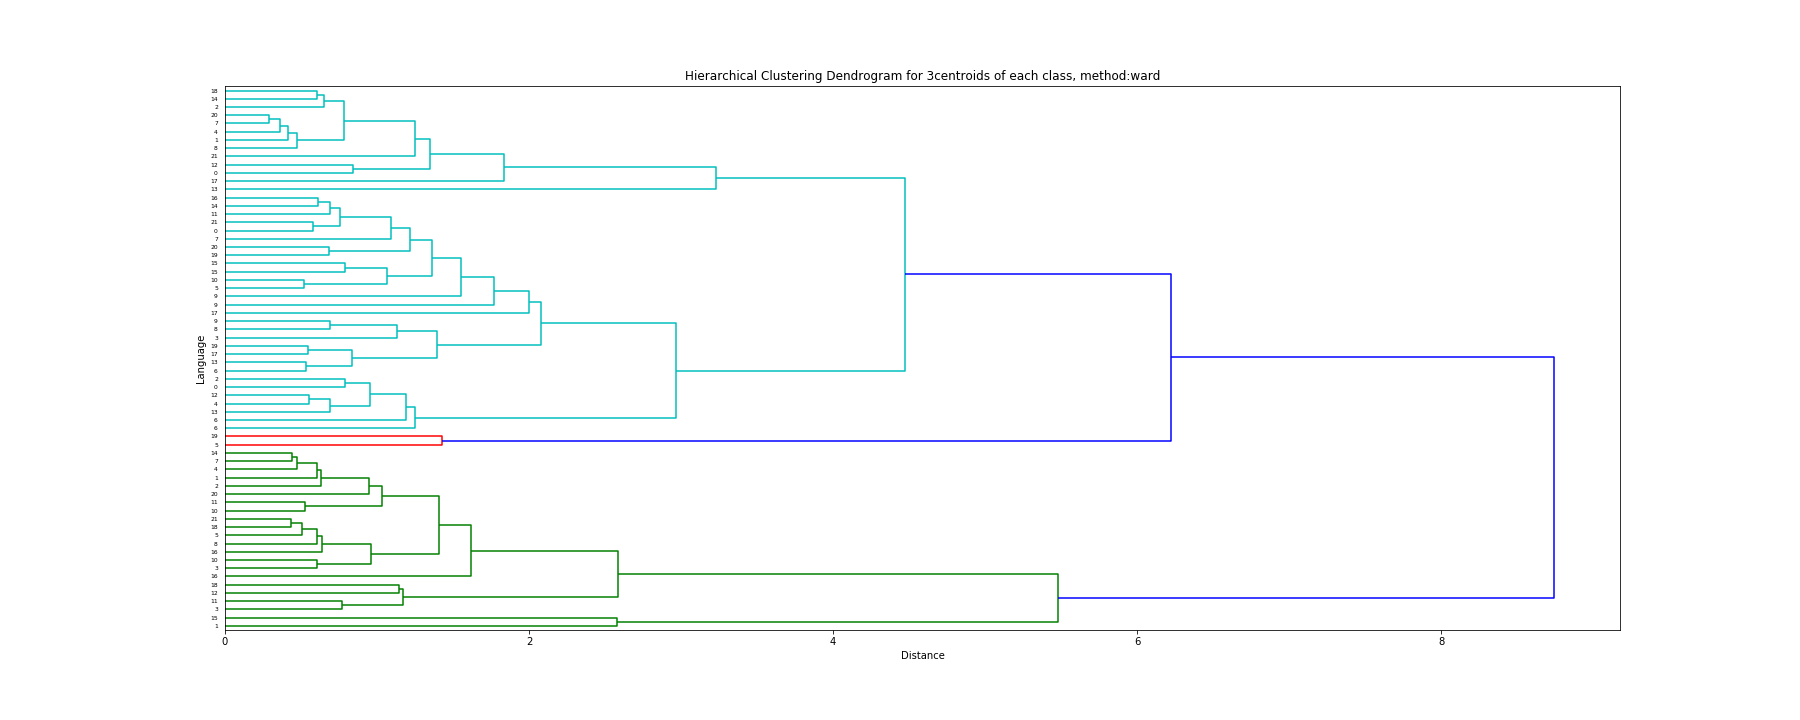
\includegraphics[width = 1.0\textwidth]{q3_4_ward.png}
         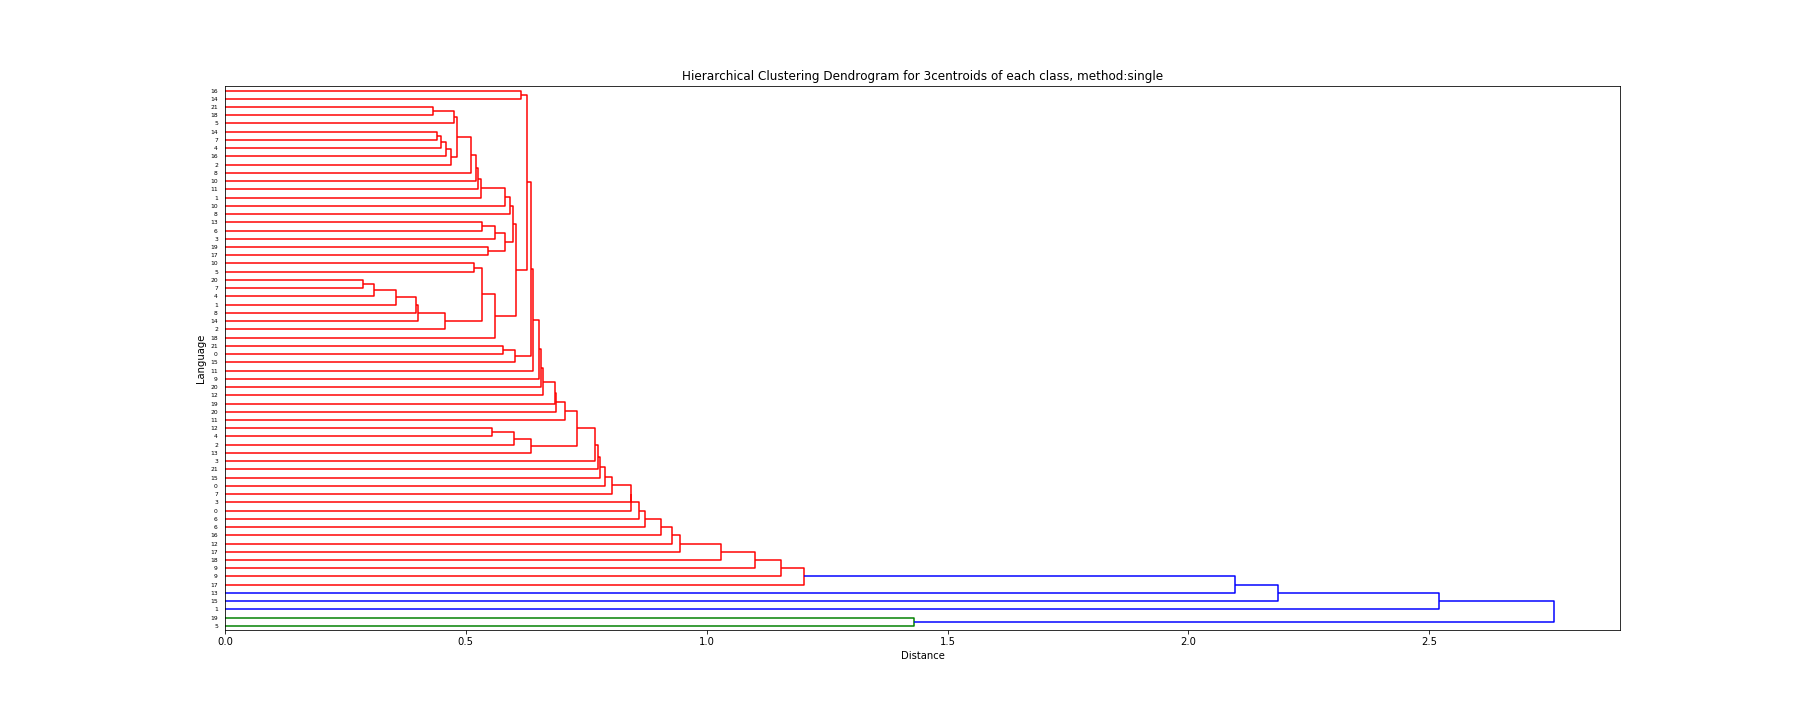
\includegraphics[width = 1.0\textwidth]{q3_4_single.png}
         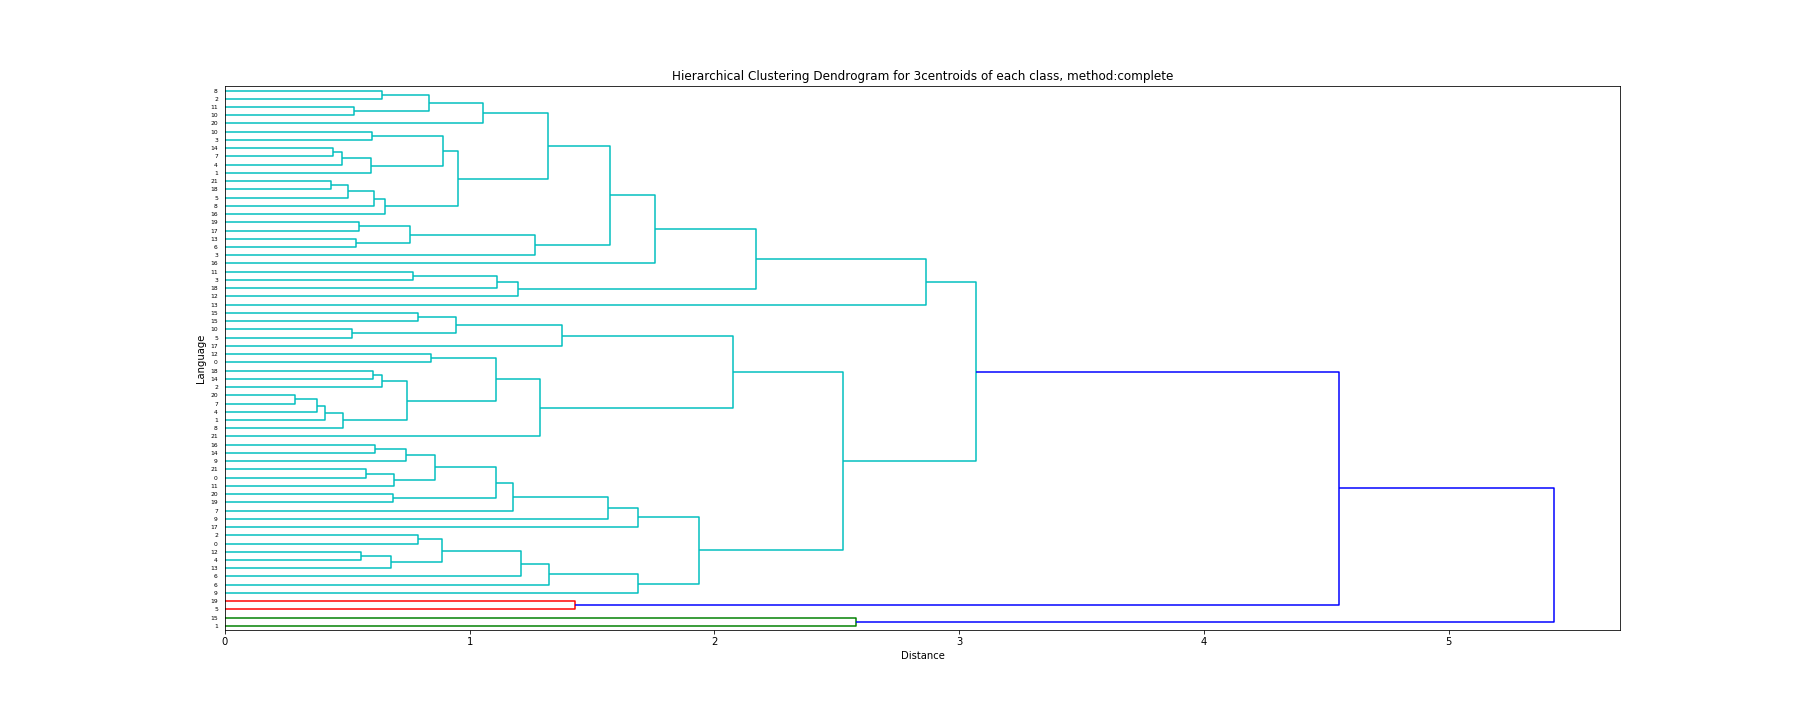
\includegraphics[width = 1.0\textwidth]{q3_4_complete.png}
         In the Ward method, most of the cluster merges happen early on. In contrast, it can be seen that the distance required for most merges to occur in the single-link method is progressive ad incremental until the distance goes beyond 1.5. Finally, in the complete-linked method most clusters are merged quite late on average.
         
         
      \end{answerbox}
  


   \end{subquestion}
   %
   % ==============================
   %
   %==============================
   % Q3.5
   \begin{subquestion}{(6 points)
       We now consider Gaussian mixture model (GMM), whose
       probability distribution function (pdf) is given as
       a linear combination of Gaussian or normal distributions, i.e.,
     } \label{Q3.5}




      \begin{answerbox}{30em}
         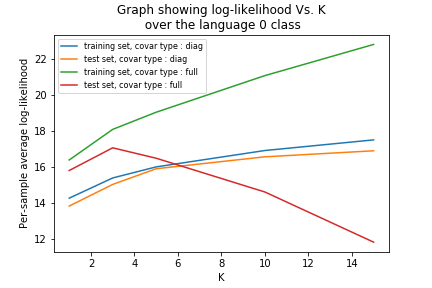
\includegraphics[width = 0.5\textwidth]{q3_5.png}
         \begin{center}
        \caption{Table showing per-sample average log-likelihoods for language 0}\newline
        \scalebox{0.85}{
        \begin{tabular}{c|c|c|c|c|c|c}
        \hline
        Data Set & covar\_type & k = 1 & k = 3 & k = 5 & k = 10 & k =15 \\ \hline
        Training & diag & 14.280 & 15.398 & 16.010 & 16.917 & 17.505 \\
        Test & diag & 13.843 & 15.041 & 15.909 & 16.568 & 16.902 \\
        Training & full & 16.394 & 18.086 & 19.036 & 21.062 & 22.786 \\
        Test & full & 15.811 & 17.066 & 16.489 & 14.622 & 11.848 \\
        \hline
        \end{tabular}}
        \end{center}
        From the graph and table above, it can be seen that when fitting a GMM with a full covariance matrix, high log-likelihoods are produced across all ranges of k on the training set. However, the model performs poorly on the unseen test data as shown by the red line. This means the GMM has been over-fit to the training data. In comparison, for a GMM trained using a diagonal covariance matrix, consistent log-likelihood performance results are obtained acroos both training and test sets, so the GMM model is a lot more suitable with this metric.
      \end{answerbox}
  


   \end{subquestion}
   %
   %==============================

   % ==============================
   
\end{question}
\end{document}
